\section{Discussion}
This section will discuss the findings from the interview study. For problems that were mentioned in the user tests, a possible solution will be discussed. For motivational factors, ways to further improve these factors will be taken into consideration.

\subsection{Hindering factors: missing interface components}
In this subsection, problems that can be solved with additional interface components will be discussed.

\subsubsection*{Overview of currently set filters}
Multiple participants had trouble recognizing what data filters were applied for the current visualization. The idea that the filters can be changed on top of the notebook and will then influence the rest of the visualization does not seem to work, especially on smaller laptops, as this resulted in a lot of scrolling.

\begin{figure}[htbp]
    \fbox{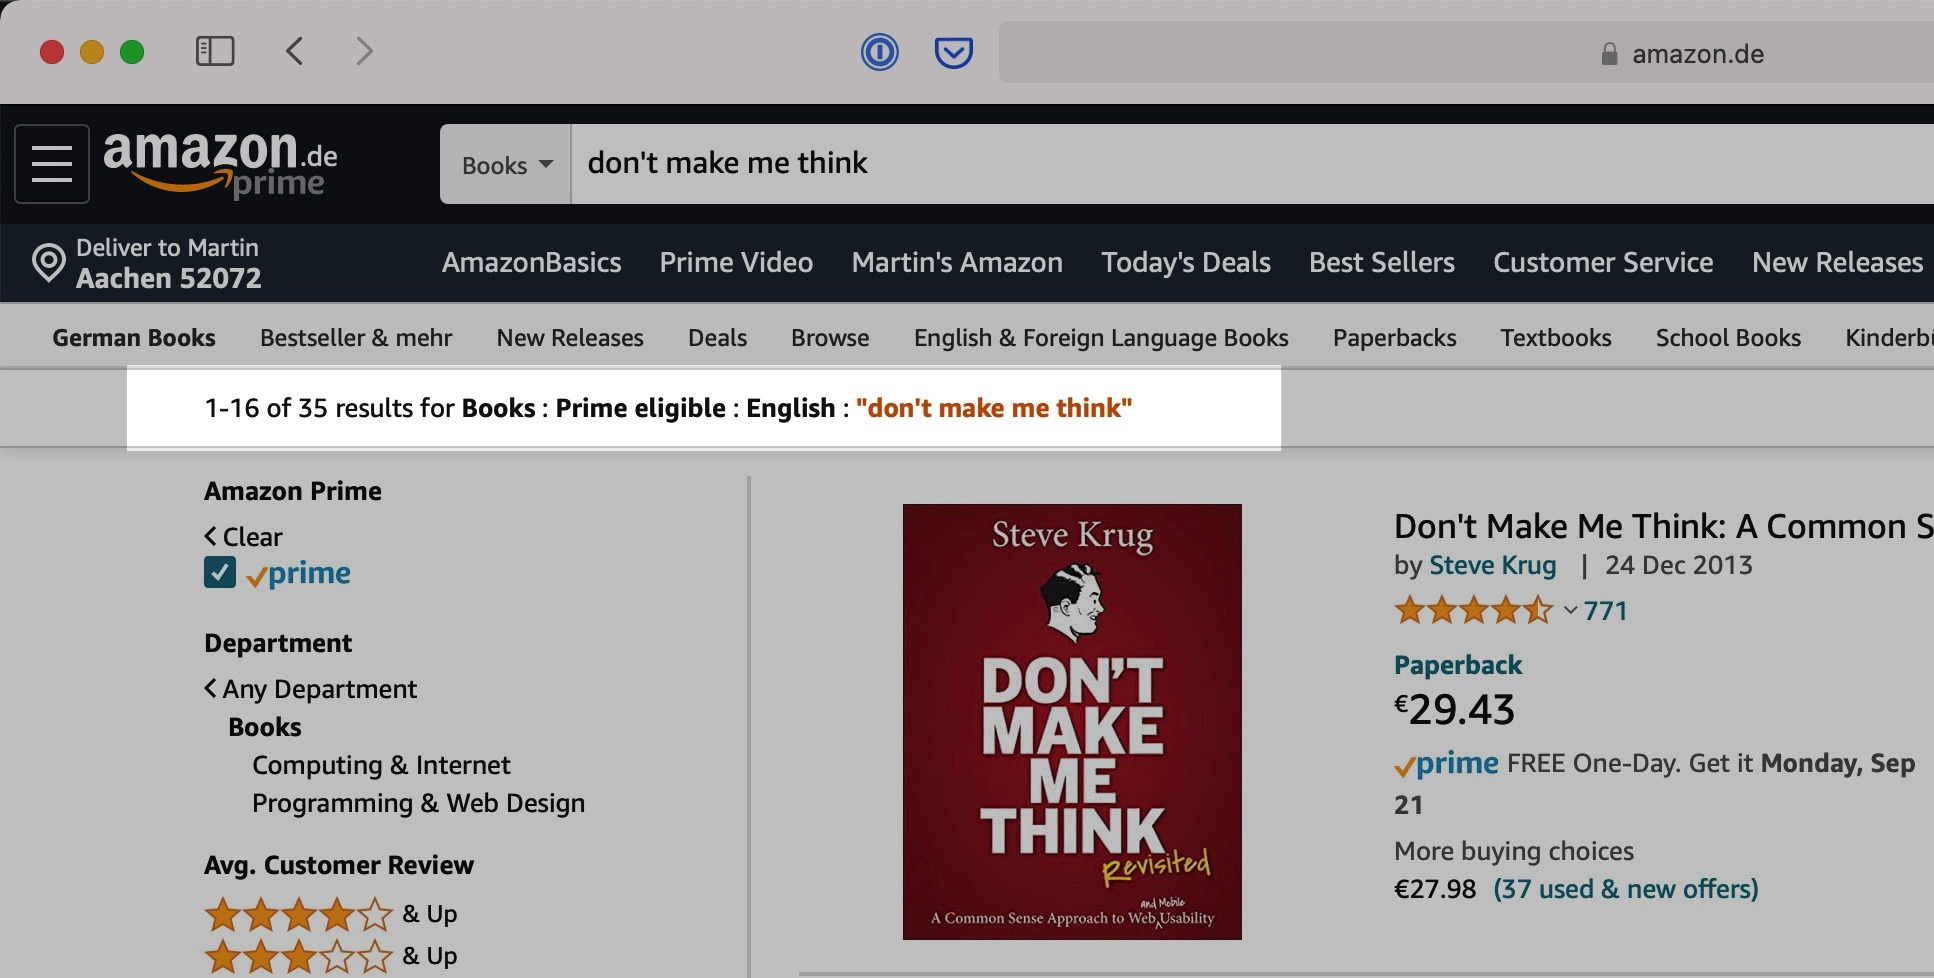
\includegraphics[width=\linewidth]{images/amazon_filters.jpg}}
    \caption{The Amazon search is filtered to English-language books which are eligible to prime-shipping, with the search input \emph{don't make me think}}
    \label{fig:amazon_filters}
\end{figure}

This means that the filter status should be visible directly next to the visualization. This way, participants would not need to search for the current filter status. Rather, the status would almost always be in view while interpreting the visualizations. There are two possible ways to show the filters near the visualizations:
\begin{enumerate}
    \item \textbf{Show a descriptive text above the visualization:} using a text to show the status of the filter could help participants to quickly understand what kind of data the visualization is showing at the moment. One example of this technique can be found on Amazon, as seen in figure \ref{fig:amazon_filters}. This technique is especially useful when a lot of different filters can be applied.
    \item \textbf{Show the filter toggles right next to the visualization:} instead of showing the filter status as a text, showing them with the actual toggles would allow users to change the filters right next to the visualization.
\end{enumerate}

\begin{figure}[h!tbp]
    \fbox{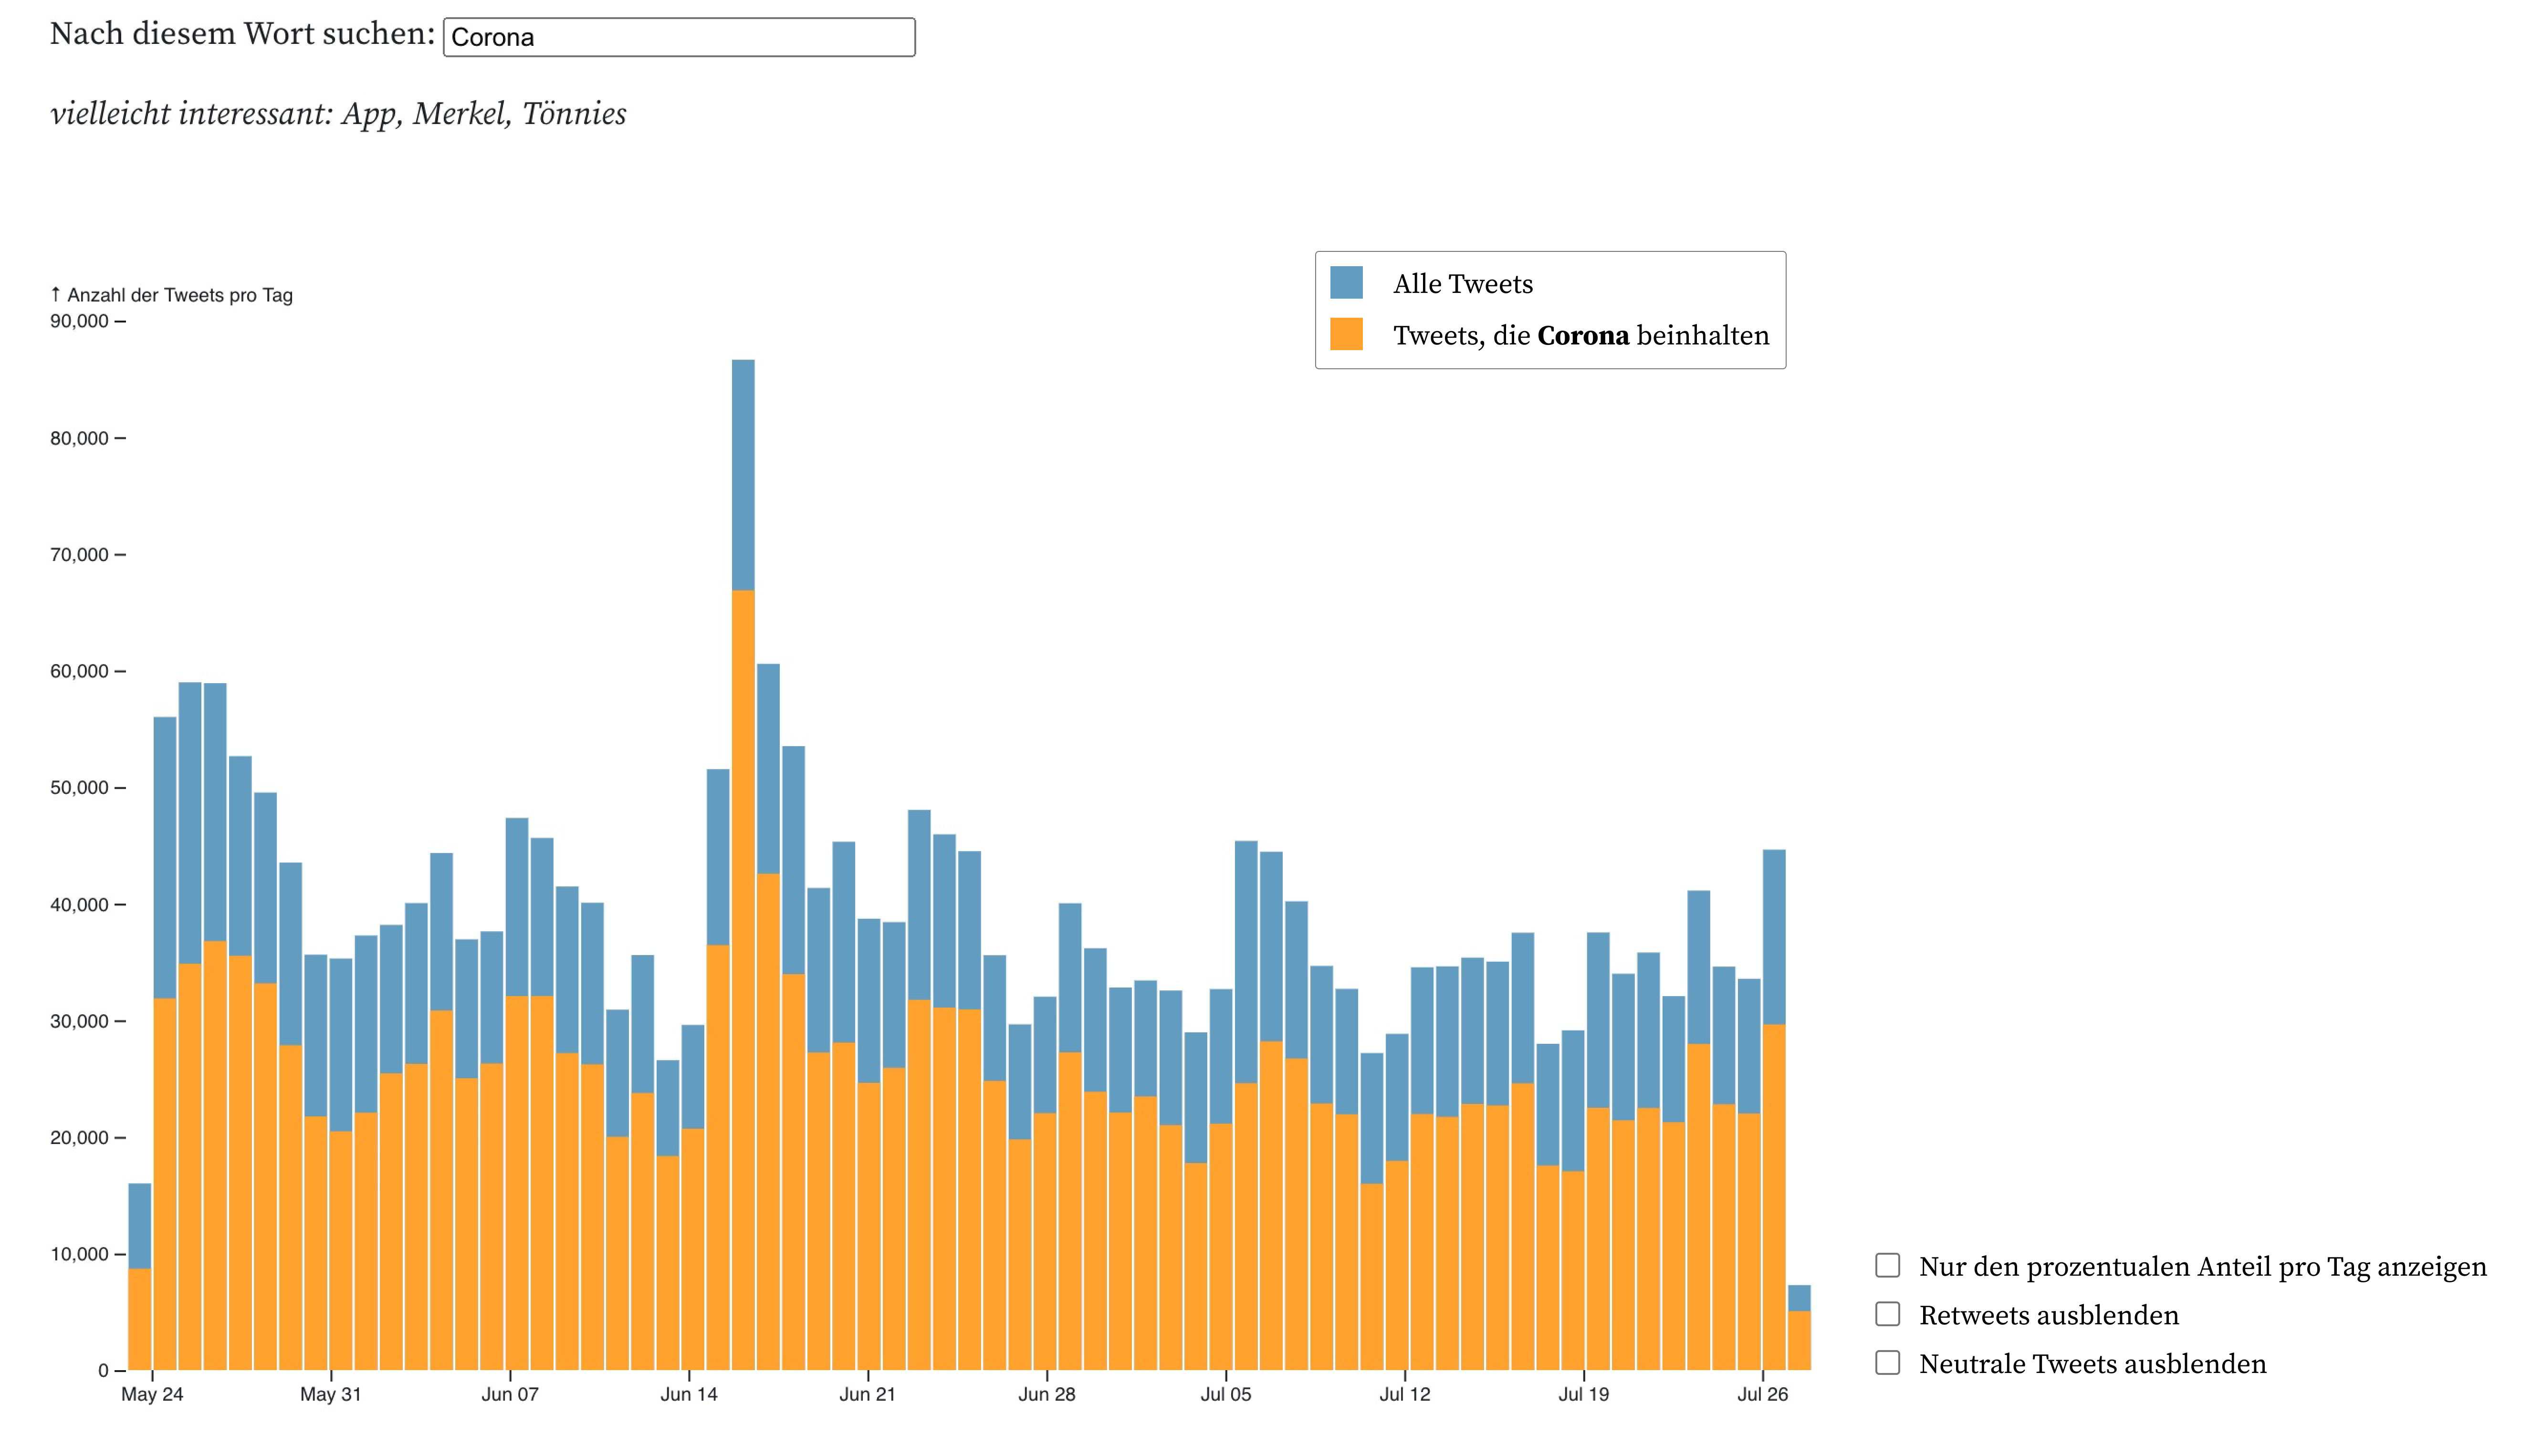
\includegraphics[width=\linewidth]{images/legend_and_filters.png}}
    \caption{Proposed layout of the tweet volume with a legend and filters directly next to the graph}
    \label{fig:legend_and_filters}
\end{figure}

Showing the filter toggles right next to the visualizations seems like a straightforward idea. However, this raises the question if the filters of the two visualizations should be linked or not, i.e., should the filter of the sentiment graph change as well when the filter of the volume graph is changed or not. To decide this, further studies should be conducted to see if the synchronicity of the data visualizations is helpful or not. This study did not examine if it helps users to have a single filter context with several visualizations or not. During the exploration phase in the interview, however, the participants did not seem to switch a lot between the tweet volume and the sentiment chart. This could suggest that having a single filter applied to both visualizations is not a necessity. In this case, using two filter sets that are independant from each other could avoid user confusion as only explicit user actions have an influence on the visualzation.

\subsubsection*{Color legend}
Another missing interface component are colored legends. During user testing, several problems arose because of the missing legend. For one, the graph was less self-contained. Users were forced to read the explanatory texts that accompanied the graph to be able to understand what the different colors mean. Another problem with the textual explanation of colors was that different participants would have named the colors differently than the text did. A legend like the one shown in figure \ref{fig:legend_example} could have helped identifying the colors more easily, as well as making the graph more self-explanatory.

Figure \ref{fig:legend_and_filters} shows a proposed addition to the tweet volume-graph. Implementing these changes makes the current filter status more obvious and lets users toggle the different filters without needing to scroll to the top of the notebook again. The legend with dynamic labelling, which includes the search term the user entered, makes the graph more self-contained.

The added legend could also help solve the layout problem that participants mentioned. With the explanatory texts no longer neccessary to understand the graphs, the texts serve as additional explanation and, as such, can remain below the graph itself.

\subsubsection*{Loading indicator}
Another component that was missing from the interface was an indicator that new data was fetched from the server. One possibility to show this fetching would be to show a small loading indicator next to the word filter. This, however, could be not visible enough. Another possiblity would be to show in the visualizations themselves that new data is being fetched. As fetching takes about 5 seconds and the visualzations have not been updated before the fetching is complete, it should not be a big problem to visually hide the visualizations during the fetching stage. A possible solution for this can be seen in figure \ref{fig:fetching_state}.

\begin{figure}[htbp]
    \fbox{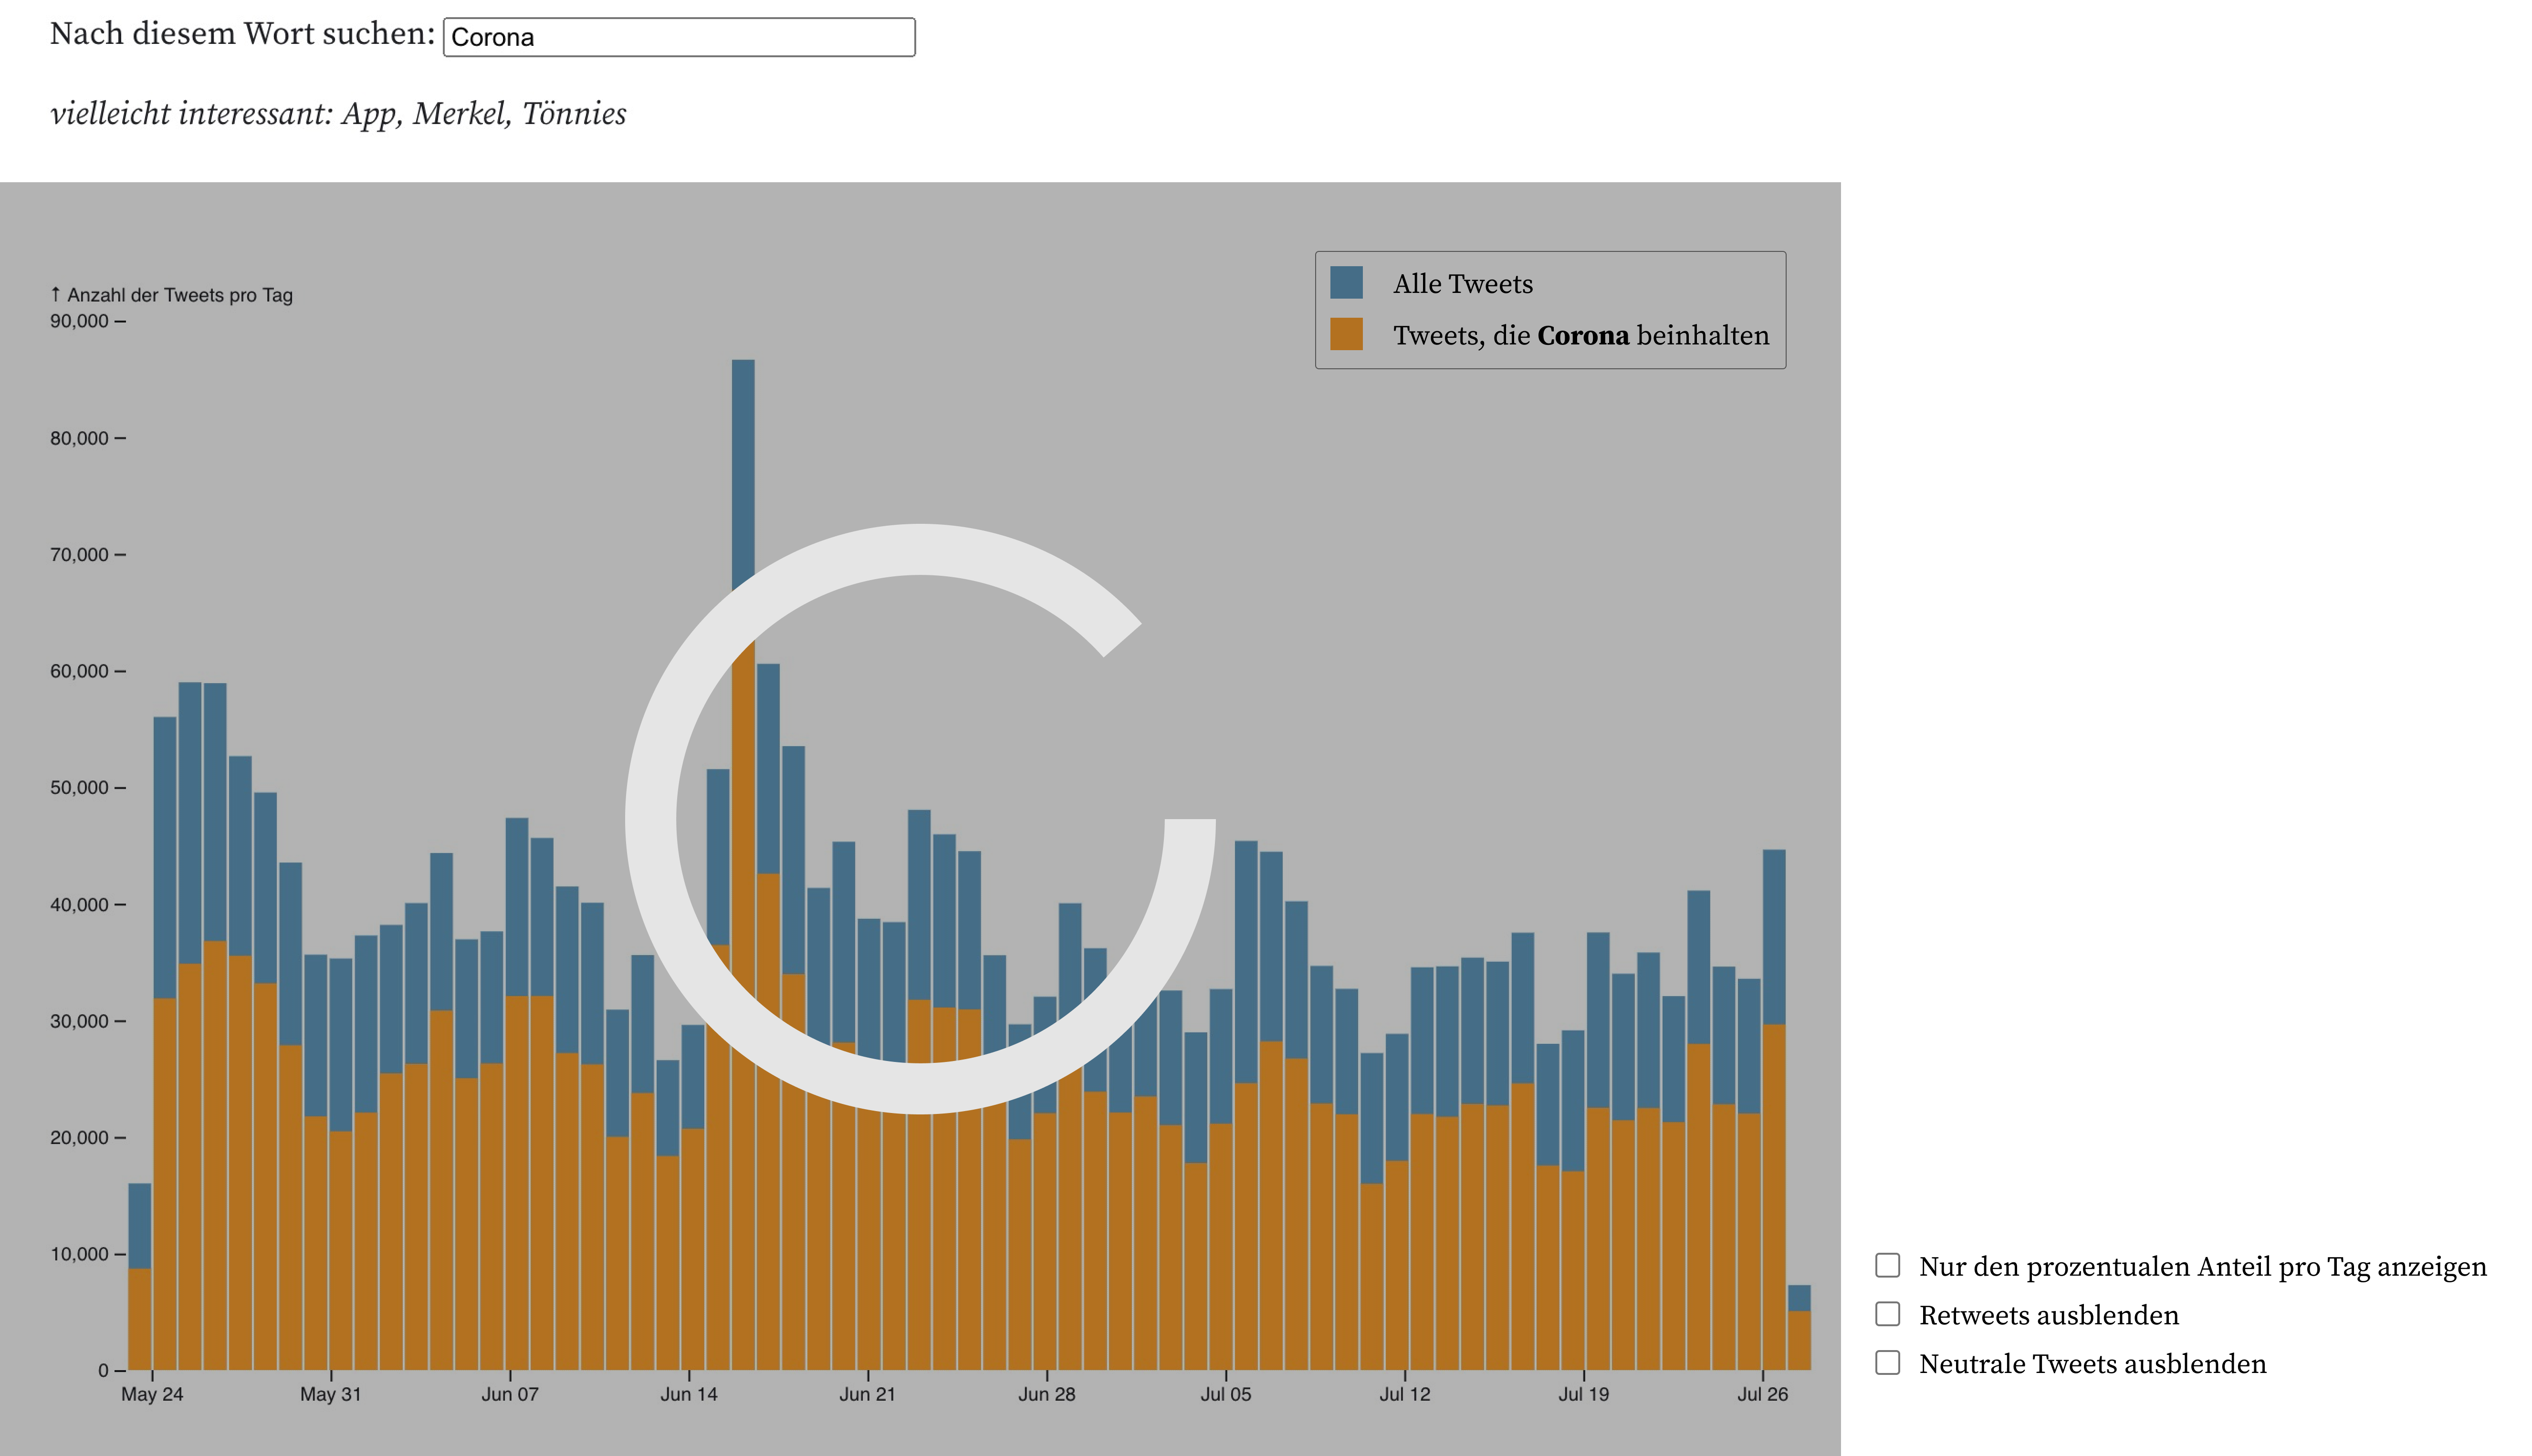
\includegraphics[width=\linewidth]{images/fetching_state.png}}
    \caption{Proposed solution to show that new data is being retrieved from the server}
    \label{fig:fetching_state}
\end{figure}

TODO: Fehlende Tooltips am Linechart ergänzen

\subsection{Technical limitations}
This section discusses findings from the interview where technical limitations hindered participants from solving tasks.

\begin{enumerate}
    \item Wort-Filter muss exakt eingegeben werden
    \item Fester Zeitrahmen der Ergebnisse
    \item Notebook-Funktionalität?
\end{enumerate}